\subsection{Steinerovy systémy trojic}
% 5 predn

\begin{definition}[Steinerův systém trojic]
    Steinerův systém trojic je $(v,k=3,\lambda=1)$-BIBD, značíme STS($v$).
\end{definition}

\begin{theorem}[Existence STS a počet prvků]
    Existuje-li STS($v$), pak $v\equiv 1$ nebo $v\equiv 3$ modulo 6.
\end{theorem}
\begin{proof}
	Z věty o parametrech BIBDu \cref{bibd_struct}:
	\[ r = \frac{\lambda (v - 1)}{k - 1} = \frac{v - 1}{2} \in \Z \Rightarrow v \equiv 1 \mod 2 \]
	Taky
	\[ |\B| = \frac{\lambda v (v - 1)}{k(k - 1)} = \frac{v (v - 1)}{6} \in \Z \Rightarrow v \not\equiv 5 \mod 6 \Rightarrow v \equiv 3 \mod 6 \]
\end{proof}

\begin{definition}[Komutativní idempotentní kvazigrupa (KIK)]\label{kvgr}
	Je teměř grupa ale operace nemusí být asociativní, nemusí existovat $e$.
	Splňuje:
    \begin{itemize}
        \item komutativní: $xy=yx$
        \item idempotentní: $xx=x$
        \item kvazigrupa: $xy=xz\Rightarrow y=z$
    \end{itemize}
\end{definition}

\begin{theorem}[STS a speciální kvazigrupa]
    STS($v$) existuje, právě když existuje komutativní idempotentní kvazigrupa na $v$ prvcích splňující \cref{kvgr} a $x(xy)=y$.
\end{theorem}
\begin{proof}
	"$\Rightarrow$". Nechť $(V, \F)$ je STS.
	Definujme binarní operaci:
	\[ xy = \twopartdef{x}{ x = y, \text{idempotence}}{z}{x \ne y \& \{ x, y, z\} \in \F} \]
	Vezmeme jednoznačný prvek ve stejné 3ci jako $x, y$.

	Zkontrolujeme vlastnosti operace:
    	\begin{itemize}
    	    \item komutativní: vždy bereme prvek z 3ci, je jedno jestli se ptáme na $xy$ nebo $yx$.
    	    \item idempotentní: z definice
	    \item podmínka $x(xy)=y$:\\
		    $x = y \Rightarrow x(xx) = xx = x$.\\
		    $x \ne y \Rightarrow x(xy) = xz = y$.
	    \item kvazigrupa: Nechť $xy = xz$ \\
		    $ x = y \Rightarrow x = z \Rightarrow x = y \Rightarrow y = z$\\
		    $x \ne y$, nechť sporem $y \ne z$ pak bychom měli 2 3ce které sdílí 2 prvky.
		    Spor s STS.
    	\end{itemize}

	"$\Leftarrow$". Máme kvazigrupa $(V, \cdot)$, definujme 3ce:
	\[ \F = \{ \{ x, y , x\cdot y \} | x \ne y \in V \} \]
	Ověříme axiomy:
	\begin{enumerate}
		\item $\F \subset \binom{V}{3}$. Nechť sporem $x\cdot y = y \Rightarrow yx = y$.
			Pak ale $y(yx) = yy \stackrel{idempotence}{=} y = x$ spor.
		\item Vezmeme libovolnou 3ci dle definice $\F$.
			Nechť sporem máme další prvek $xy = z$ který tvoří další 3ci:
			\[ \{ x, z, xz \} = \{ x, z, x(xy) = y \} = \{ x, z, y \} \]
	\end{enumerate}
\end{proof}
\begin{theorem}[Kombinace STS]
    $\forall v_1,v_2: \exists$ STS($v_1$), STS($v_2$)$\Rightarrow\exists$ STS($v_1\cdot v_2$).
\end{theorem}
\begin{proof}
	Nechť máme $(V_1, \circ_1)$ a $(V_2, \circ_2)$ splňující \cref{kvgr} a $x(xy)=y$.
	Pak kartezský součin s operaci definovanou po složkách je algebra stejného typu
	\[ (V_1, \circ_1) \times (V_2, \circ_2) = (V_1 \times V_2, \circ), (a, b) \circ (x, y) = (a \circ_1 x, b \circ_2 y) \]
	% overeni vypoctem, predn 5 od 21:00
\end{proof}

\begin{consequence}[STS(9)]
	$\exists$ STS(9) $=$ STS(3) $\times$ STS(3).

	Sice STS(3) na 3-prvkové množině by nesplňoval $v \ne k$ ale z historických důvodu ho považujeme za validní.
	Stejně tak STS(1) (jeden prvek).
\end{consequence}

\begin{exercise}[$\exists$ STS(15)?]
\end{exercise}

\begin{theorem}[Nutná podmínka je i postačující pro STS]
    $\forall v\equiv 1, v\equiv 3\mod 6, \exists$ STS($v$).
\end{theorem}
\begin{proof}[Důkaz pro 3, Boseho konstrukce]
	$V = \Z_{2m + 1} \times \Z_3$, pak 3ce budou
	\[ \F = \{ \{(i, 0), (i, 1), (i, 2) \}| i \in \Z_{2m + 1} \} \cup \{ \{ (i, k), (j, k), ((m+1)(i + j), k + 1) \} | i \ne j \in \Z_{2m + 1}, k \in \Z_3 \} \]

	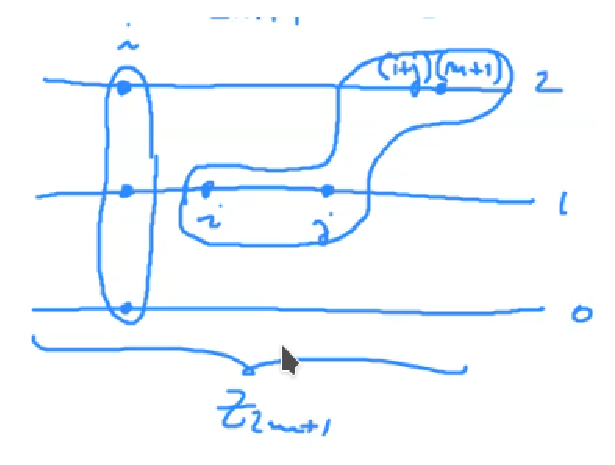
\includegraphics[scale=0.5]{3c_0.eps}

	\begin{enumerate}
		\item \# prvků $|V| = (2m + 1)3 = 6m + 3 \equiv 3 \mod 6$.
		\item \# 3c
			\[ |\F| = 2m + 1 + 3 \binom{2m + 1}{2} = 2m + 1 + 3 \cdot \frac{(2m + 1)2m}{2} = 6m^2 + 5m + 1 = \]
			\[ = (3m + 1)(2m + 1) = \frac{1}{6} (6m + 3)(6m + 2) = \frac{1}{6} |V|(|V| - 1) \]
			Zbývá zkontrolovat, že pro libovolnou 3ci prvků máme množinu.
			Zkontrolujeme 3ce rozborem případu
			\begin{enumerate}
				\item prvky jsou v různých řádcích ale nad sebou.
					Pak existuje množina z první podmínky.
				\item prvky jsou ve stejném řádku.
					Pak existuje množina z druhé podmínky.
				\item prvky jsou v různých řádcích ale ne nad sebou, na pozicích $(j, k), (h, k + 1)$.
					Pak hledáme $i: h = (m + 1)(i + j) \iff 2h = (2m + 2)(i + j) = i + j \iff i = 2h - j$.
					Z vlastnosti okruhu takové $i$ je jednoznačné.
					Musíme zkontrolovat $i \ne j$.

					Nechť sporem $i = j \Rightarrow 2j = 2h \Rightarrow j = h$.
					Spor s volbou prvku z různých řádků.

				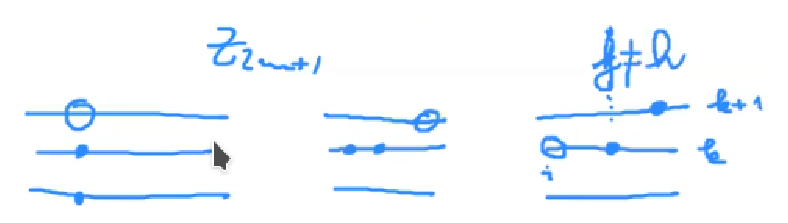
\includegraphics[scale=0.5]{3c_1.eps}
			\end{enumerate}
	\end{enumerate}
\end{proof}
\begin{proof}[Důkaz pro 1, Skolemova konstrukce]
	$v = 6m + 1$.
	Nechť
	\[ V = \Z_{2m} \times \Z_3 \cup \{w\} \]
	Představujeme $\Z_{2m} = \{ 1, \ldots, 2m = 0 \}$.
	\begin{gather*}
		\F = \{ \{ (i, 0), (i, 1), (i, 2) \}| i \in [m] \} \cup \\
		     \{ \{ (i, k), (i + m, k - 1), w \} | i \in [m], k \in [3] \} \cup \\
		     \{ \{ (i, k), (j, k), (L_{i, j}, k + 1) \} | i \ne j \in \Z_{2m}, k \in [3] \}
	\end{gather*}

	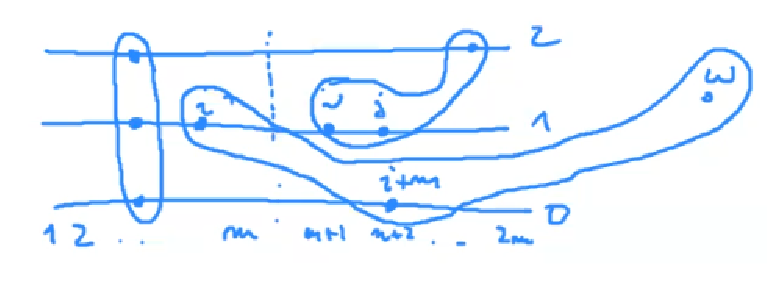
\includegraphics[scale=0.6]{3c_2.eps}

	Kde $L \in Z_{2m}^{2m \times 2m}$ je \emph{symetrický} Latinský čtverec takový, že na diagonále má dvakrát posloupnost $1, \ldots, m$:
	\[ L_{i, i} = L_{m + i, m + i} = i, i \in [m] \]
	Potřebujeme symetrický LČ protože 3 podmínka množiny musí být stejná nezávislé na tom, jestli se ptáme na $i, j$ nebo $j, i$.

	\begin{enumerate}
		\item \# prvků $|V| = 6m + 1 \equiv 1 \mod 6$.
		\item \# 3c, sčítance odpovídají typům množin v definici
			\[ |\F| = m + 3m + 3 \binom{2m}{2} = 4m + 3 \cdot \frac{(2m - 1)2m}{2} = 6m^2 + m = \]
			\[ = \frac{1}{6} (6m + 1) 6m = \frac{1}{6} |V|(|V| - 1) \]
			Zbývá zkontrolovat, že pro libovolnou 3ci prvků máme množinu.
			Zkontrolujeme 3ce rozborem případu
			\begin{enumerate}
				\item jeden z prvků je $w$ a druhý prvek je v první půlce $\in [m]$.
					Pak třetí prvek v druhé půlce o řád dole.
				\item jeden z prvků je $w$ a druhý prvek je v druhé půlce $\in \{ m, \ldots, 2m \}$.
					Pak třetí prvek v druhé půlce o řád nahoře v první půlce.
				\item prvky jsou ve stejném řádku.
					Pak existuje množina z třetí podmínky.
				\item prvky jsou v různých řádcích ale nad sebou v první polovině.
					Pak existuje množina z první podmínky.

				
\includegraphics[scale=0.6]{3c_3.eps}
				\item prvky jsou v různých řádcích ale nad sebou v druhé polovině.
					Chceme $\exists i: L_{i, j} = j \& i \ne j$.
					Z vlastnosti LČ $i$ je jednoznačné a nemůže se rovnat $j$ protože v druhé polovině na $j$-té pozice je prvek $j - m \ne j$.
				\item prvky jsou v různých řádcích ale ne nad sebou, na pozicích $(j, k), (h, k + 1)$.
					Chceme $\exists i: h = L_{i, j}$.
					Z vlastnosti LČ $i$ je jednoznačné, chceme znovu $i \ne j$.
					Nechť sporem $i = j$, pak jsme na diagonále.

					Pokud $j > m \Rightarrow h = j - m \ne j$.
					Opačně, $j \leq m \Rightarrow i = j = m$, což je již vyřešený případ v d).

				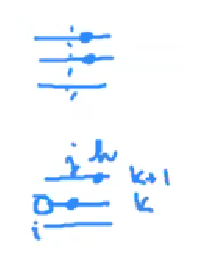
\includegraphics[scale=0.6]{3c_4.eps}
				\item prvky na pozicích $(h = j - m, k + 1)$ a $(j, k)$.
					Pak ale $j = i$ a případ pokrývá 3ce s $w$.
				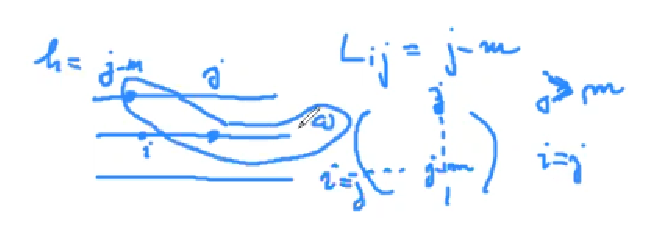
\includegraphics[scale=0.6]{3c_5.eps}
			\end{enumerate}
	\end{enumerate}

\end{proof}

% predn 5 od 01:00:00
\begin{proof}[Obecný \uv{tabulkový} důkaz]
	% todo predn 5 od 01:04:00
	\begin{lemma}[Tabulkový důkaz 1]
		$\exists STS(v_1) = S_1, STS(v_2) = S_2, STS(v_3) = S_3: S_3 \subseteq S_2 \Rightarrow \exists S = STS(v_3 + v_1(v_2 - v_1)) $
		Navíc obsahuje původní jako podsystémy: $ \simeq S_i \subseteq S, i \in [3]$.
	\end{lemma}
	\begin{proof}
		Označme $t = v_2 - v_3$.
    		TODO
	\end{proof}

	\begin{lemma}[Tabulkový důkaz 2]
		$\exists$ STS(v) $\subseteq$ KPR(2) (Fanová rovina) $\Rightarrow \exists$ STS($f(v)$) který taky obsahuje Fanovu rovinu, kde $f$ je specifikovaná dle pravidel:
		\begin{enumerate}[label=\alph*)]
			\item $v_1 = v, v_2 = 3, v_3 = 1 \Rightarrow 1 + v (3 - 1) = 2v + 1$
			\item $v_1 = 3, v_2 = v, v_3 = 1 \Rightarrow 1 + 3(v - 1) = 3v - 2$
			\item $v_1 = 3, v_2 = v, v_3 = 3 \Rightarrow 3 + 3(v - 3) = 3v - 6$
			\item $v_1 = v, v_2 = 9, v_3 = 3 \Rightarrow 3 + v(9 - 3) = 6v + 3$
			\item $v_1 = 3, v_2 = v, v_3 = 7 \Rightarrow 7 + 3 (v - 7) = 3v - 14$
			\item $v_1 = v, v_2 = 7, v_3 = 1 \Rightarrow 1 + v(7 - 1) = 6v + 1$
		\end{enumerate}
		Předpoklad o Fanové rovině potřebujeme pouze pro e).
	\end{lemma}
	\begin{proof}
		Ověříme, že $\forall v \equiv 1 \lor 3 \mod6$ pokud $v \leq 1944 \exists$ STS(v), pak pokud $v \geq 325 \exists$ STS(v)$\supseteq$ KPR(2).

		Indukci dokážeme $\forall v \equiv 1 \lor 3 \mod6$ pokud $v \leq 1944 \exists$ STS(v)$\supseteq$ KPR(2).
		Rozbor případů dle $v \mod36$, napíšeme $v = 36t + z$.
		% todo upravit dle handout 5
		Taky $1944 = 36 \cdot 54 \Rightarrow t \geq 54 \Rightarrow 6t \geq 324$.

		% todo aplikace pravidel dle handout 5

	\end{proof}
\end{proof}
